\documentclass[a4paper]{jarticle}
\usepackage{comment}
\usepackage{slashbox}
\usepackage{listings,jlisting}
\usepackage[dvipdfmx]{graphicx}
\usepackage[top=20truemm,bottom=20truemm,left=20truemm,right=20truemm]{geometry}
\title{計算機工学実験A課題3レポート}
\author{学生番号 氏名}
\date{2016/11/24}
\lstset{%
	basicstyle={\small},%
	tabsize=8,
	identifierstyle={\small},%
	commentstyle={\small\itshape},%
	keywordstyle={\small\bfseries},%
	ndkeywordstyle={\small},%
	stringstyle={\small\ttfamily},
	frame={tb},
	breaklines=true,
	columns=[1]{fullflexible},%
	numbers=left,%
	xrightmargin=0zw,%
	xleftmargin=3zw,%
	numberstyle={\scriptsize},%
	stepnumber=1,
	numbersep=1zw,%
	lineskip=-0.5ex,%
	keepspaces=true,
	showstringspaces=false
}
\begin{document}
\maketitle

\begin{comment}
\section{実験の総括的な目的}
ハードウェア記述言語のSystem Verilogを使って回路を設計し、テストベンチを使ってModelSim上で回路の動作を確かめる。
\section{実験結果}
\subsection{課題1}
\subsubsection{目的}
配布された「速攻ModelSim」に記載された手順に従って、workフォルダの中にあるsyllyfunction.svの中のsillyfunctionの動作を、三種類のテストベッド$(testbench\_example1.sv,testbench\_example2.sv,testbench\_example3.sv)$を使ってModelSim上で試す。
\subsubsection{道のり}
workフォルダからコピーしてきたSystem Verilogのソースコードは以下の四つである。
\lstinputlisting[caption=$sillyfunction.sv$,label=work1sillyfunction]{1/sillyfunction.sv}
\lstinputlisting[caption=$testbench\_example1.sv$,label=work1testbench1]{1/testbench_example1.sv}
\lstinputlisting[caption=$testbench\_example2.sv$,label=work1testbench2]{1/testbench_example2.sv}
\lstinputlisting[caption=$testbench\_example3.sv$,label=work1testbench3]{1/testbench_example3.sv}
モジュールsillyfunctionの真理値表は表\ref{Work1TruthTable}のとおりになる。
\begin{table}[ht]
	\begin{center}
		\caption{sillyfunctionの真理値表}
		\label{Work1TruthTable}
		\begin{tabular}{|c|c|c||c|}
			\hline
			\multicolumn{3}{|c|}{入力} & \multicolumn{1}{|c|}{出力}\\ \hline\hline
			a	&b	&c	&y\\	\hline\hline
			0	&0	&0	&1\\	\hline
			0	&0	&1	&0\\	\hline
			0	&1	&0	&0\\	\hline
			0	&1	&1	&0\\	\hline
			1	&0	&0	&1\\	\hline
			1	&0	&1	&1\\	\hline
			1	&1	&0	&0\\	\hline
			1	&1	&1	&0\\	\hline
		\end{tabular}
	\end{center}
\end{table}
ModelSim上で新しいプロジェクトを作成し、これらのソースコードを加えてすべてコンパイルし、エラーが出ないことを確認した後各々のテストベッドについてシミュレーションを行い、a,b,cの値に応じてyの値が同じように振る舞うことを確認した。
\subsubsection{結果}
\begin{center}
	$testbench\_example1.sv$のシミュレーション結果
	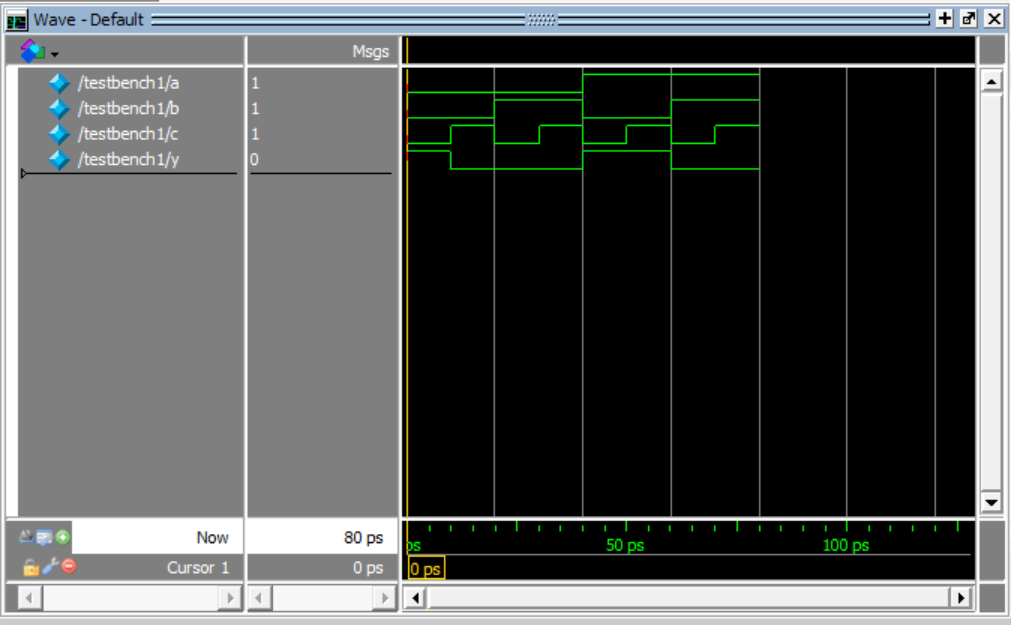
\includegraphics[width=15cm]{1-m-1.PNG}
\end{center}
\begin{center}
	$testbench\_example2.sv$のシミュレーション結果
	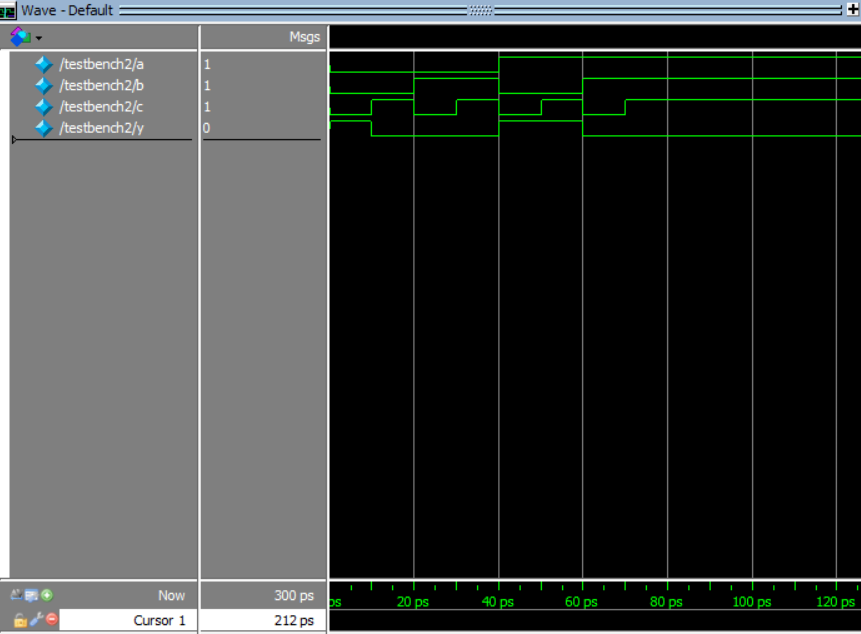
\includegraphics[width=15cm]{1-m-2.PNG}
\end{center}
\begin{center}
	$testbench\_example2.sv$によるシミュレーション時のエラー
	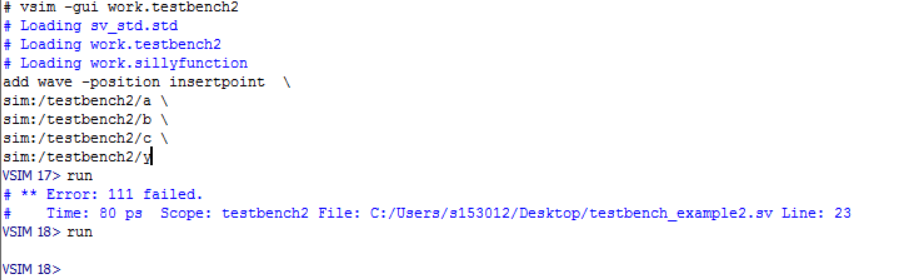
\includegraphics[width=15cm]{testbench2error.PNG}
\end{center}
\begin{center}
	$testbench\_example3.sv$のシミュレーション結果
	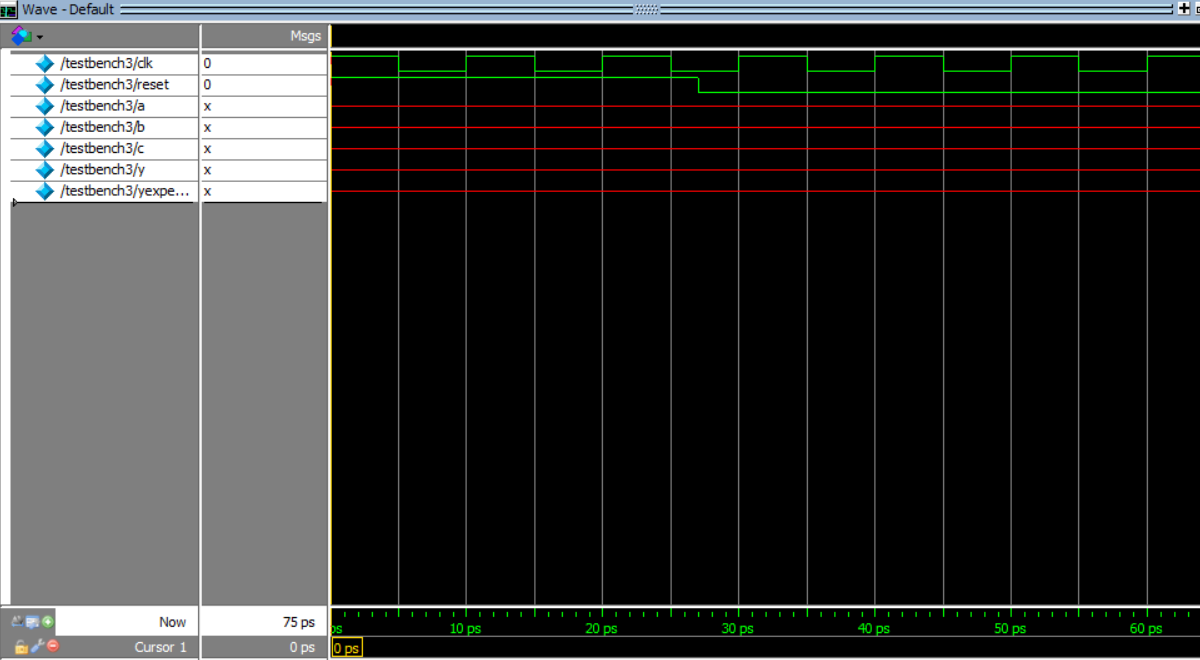
\includegraphics[width=15cm]{1-m-3.PNG}
\end{center}
上の図のように、$testbench\_example1.sv$と$testbench\_example2.sv$と$testbench\_example3.sv$のシミュレーション結果では$sillyfinction$の入力$a,b,c$に対して出力$y$は同じように振る舞ったが、$testbench\_example2.sv$によるシミュレーションでは上の図のようなエラーが表示された。
\subsubsection{考察}
ハードウェア記述言語であらわされた回路をModelSim上でシミュレーションするのはこの課題が初めてだった。新しいプロジェクトを作成し、プロジェクトにソースコードを加えてシミュレーションを行い、波形を確認するというModelSimの一連の使い方を習得することが出来た。
\subsection{課題2}
\subsubsection{目的}
課題4の用紙にある図4.11のHDL記述のコードを回路図で描く。また、ゲート数が最小になるように回路を簡単化する。
\subsubsection{道のり}
まず、課題4の用紙にある図4.11のHDL記述のコードをそのまま回路図であらわすと以下のようになる。
\begin{center}
	簡略する前の回路図
	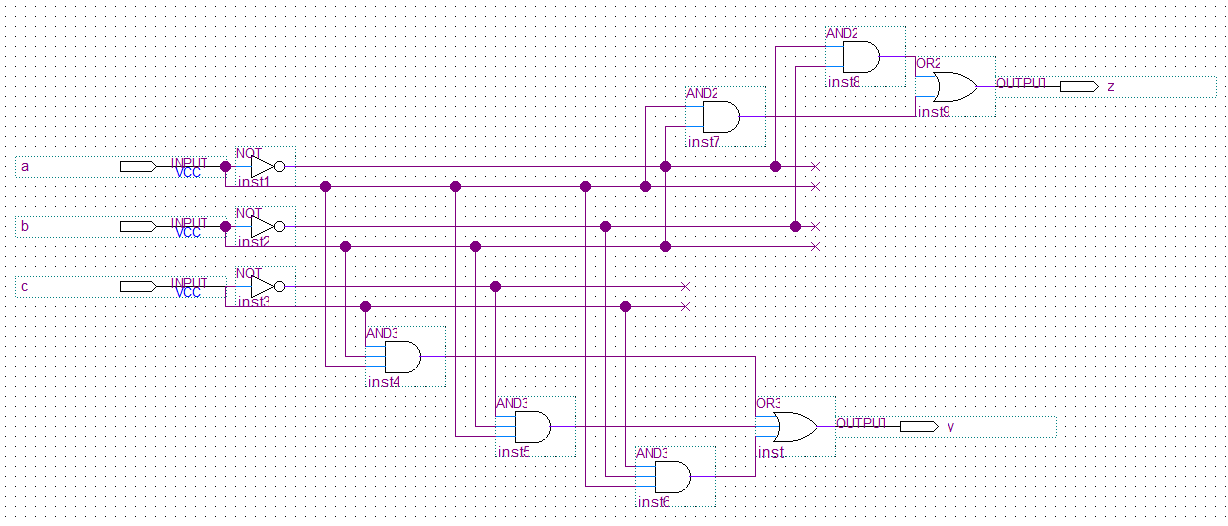
\includegraphics[width=15cm]{2-l-1.PNG}
\end{center}
そして、回路の出力$y,z$について式変形をすると、
\begin{eqnarray*}
	y & = & a \land b \land c \lor a \land b \land \tilde{c} \lor a \land \lnot b \land c \nonumber \\
	  & = & a \left( b \land c \lor b \land \lnot c \lor \left( \lnot b \right) \land c \right) \nonumber \\
	  & = & a \left( b \lor c \right) \nonumber \\
	z & = & a \land b \lor \left( \lnot a \right) \land \left( \lnot b \right) \nonumber \\
	  & = & \lnot \left( a \bigoplus b \right) \nonumber \\
\end{eqnarray*}
となる。
\subsubsection{結果}
\begin{center}
	簡略化した後の回路図
	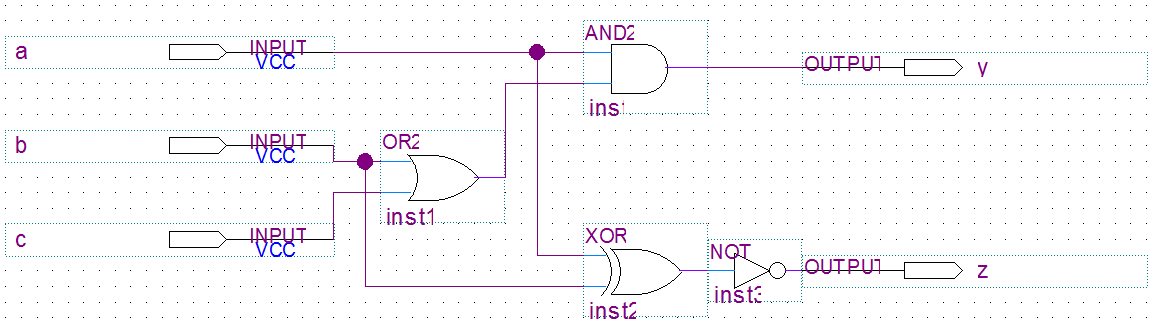
\includegraphics[width=15cm]{2-l-2.PNG}
\end{center}
\subsubsection{考察}
HDL記述から回路図を描き、さらに式変形によってゲート数を最小化することが出来た。
\subsection{課題3}
\subsubsection{目的}
4入力のXOR関数を計算するSystemVerilogのモジュールとそのテストベッドを書き、シミュレーションで検証する。
\subsubsection{道のり}
まず、複数入力のxor関数の出力は奇数個の入力が1であるとき1であるから、真理値表は以下の表\ref{Work3TruthTable}のようになる。
\begin{table}[ht]
	\begin{center}
		\caption{4入力xor関数の真理値表}
		\label{Work3TruthTable}
		\begin{tabular}{|c|c|c|c||c|}
			\hline
			\multicolumn{4}{|c|}{入力} & \multicolumn{1}{|c|}{出力}\\ \hline\hline
			a[0]	&a[1]	&a[2]	&a[3]	&y\\	\hline\hline
			0	&0	&0	&0	&0\\	\hline
			0	&0	&0	&1	&1\\	\hline
			0	&0	&1	&0	&1\\	\hline
			0	&0	&1	&1	&0\\	\hline
			0	&1	&0	&0	&1\\	\hline
			0	&1	&0	&1	&0\\	\hline
			0	&1	&1	&0	&0\\	\hline
			0	&1	&1	&1	&1\\	\hline
			1	&0	&0	&0	&1\\	\hline
			1	&0	&0	&1	&0\\	\hline
			1	&0	&1	&0	&0\\	\hline
			1	&0	&1	&1	&1\\	\hline
			1	&1	&0	&0	&0\\	\hline
			1	&1	&0	&1	&1\\	\hline
			1	&1	&1	&0	&1\\	\hline
			1	&1	&1	&1	&0\\	\hline
		\end{tabular}
	\end{center}
\end{table}
xor関数を計算するSystemVerilogのモジュールをソースコード\ref{work3sv}のように定義した。
\lstinputlisting[caption=$work3.sv$,label=work3sv]{3/work3.sv}
次に、ソースコード\ref{work3sv}に対するテストベッドをソースコード\ref{work3testbench}のように定義し、シミュレーションを実行した。
\lstinputlisting[caption=$testbench.sv$,label=work3testbench]{3/testbench.sv}
\subsubsection{結果}
シミュレーションを実行した結果、下の図のような奇数個の入力が1のときに出力が1となる波形となった。
\begin{center}
	課題3シミュレーション結果
	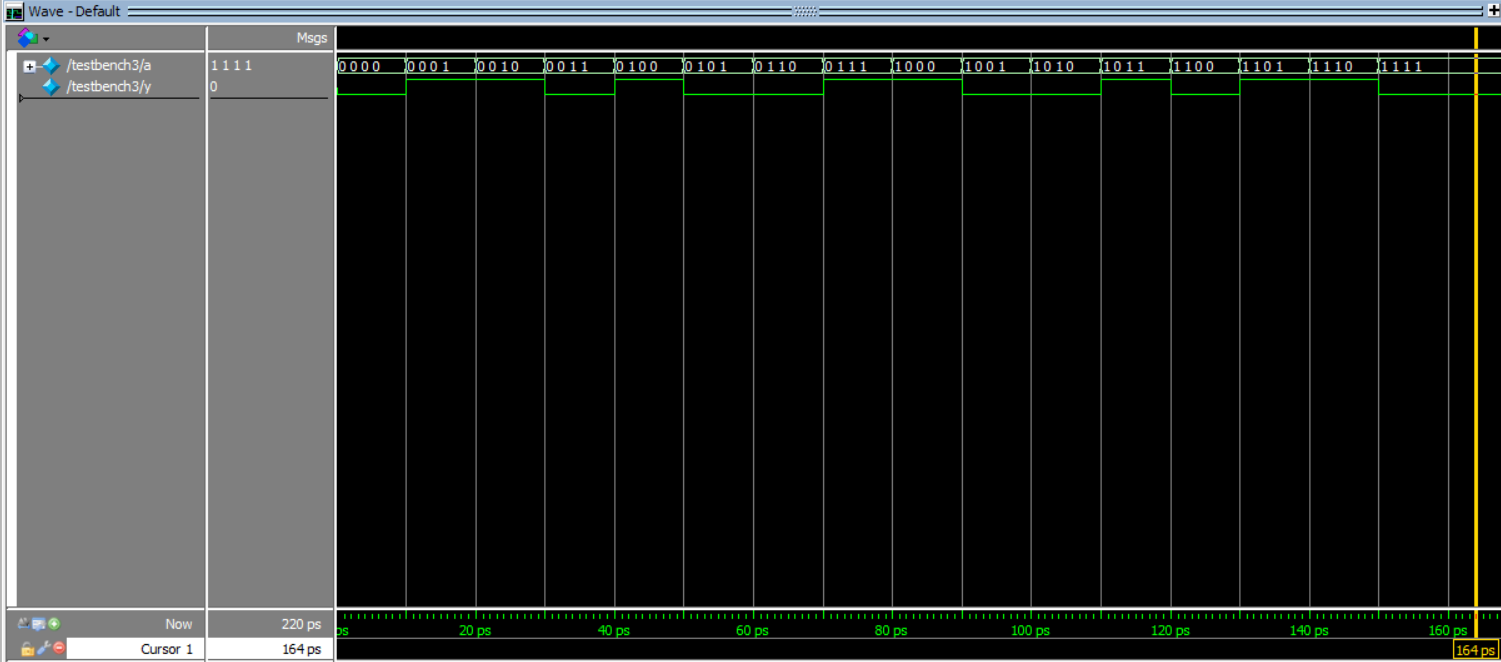
\includegraphics[width=15cm]{3-m.PNG}
\end{center}
\subsubsection{考察}
課題3ではSystemVerilogで単純な回路を設計し、それが正常に動くかどうかを確認するためにテストベッドを作ってシミュレーションを実行した。これにより、SystemVerilogで回路を設計して動作を確認する一連の手順を理解することができた。
\subsection{課題4}
\subsubsection{目的}
minorityという名のSystemVerilogモジュールとそのテストベッドを書き、シミュレーションで検証せよ。minorityは3つの入力a,b,cを受け、1つの出力yを生成する。少なくとも2つの入力がFALSEならyはTRUEになるようにする。
\subsubsection{道のり}
まず、モジュールminorityを下のソースコード\ref{work4sv}のように定義した。
\lstinputlisting[caption=$work4.sv$,label=work4sv]{4/work4.sv}
次に、そのテストベッドとして下のソースコード\ref{work4testbench}を定義し、シミュレーションを実行した。
\lstinputlisting[caption=$work4testbench.sv$,label=work4testbench]{4/work4testbench.sv}
\subsubsection{結果}
シミュレーションを実行した結果、下の図のように入力a,b,cのうち少なくとも2つがFALSEならば出力yがTRUEになる波形が得られた。
\begin{center}
	課題4シミュレーション結果
	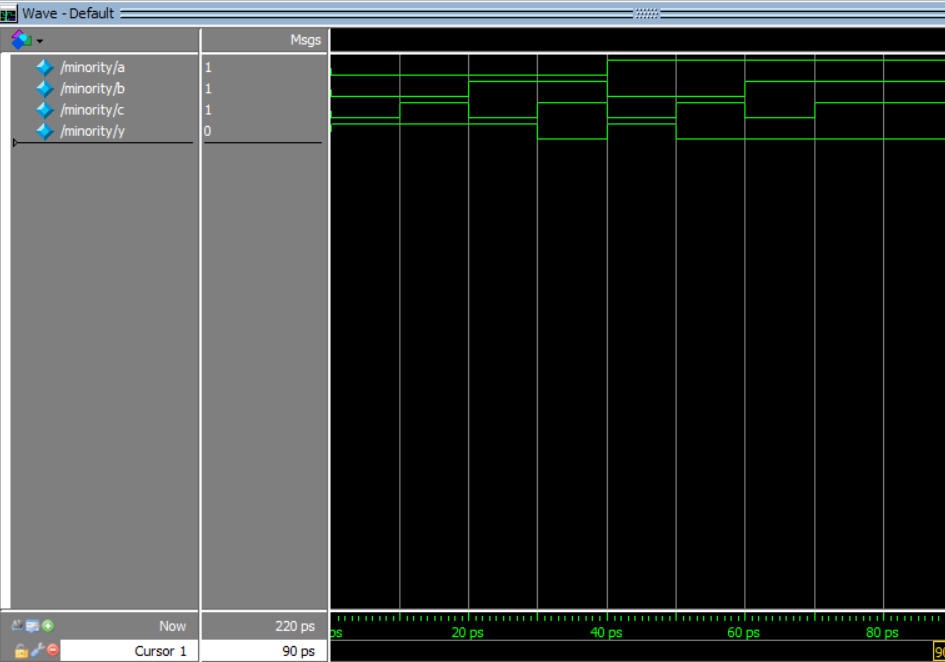
\includegraphics[width=15cm]{4-m.PNG}
\end{center}
\subsubsection{考察}
課題4では、目的にあった回路を作成するために、論理式を立ててそれを元にSystemVerilogでモジュールを定義してシミュレーションで動作を確認した。また、モジュールの入力で課題3とは異なり配列を使わずに複数の入力を受け付ける方法を知った。
\subsection{課題5}
\subsubsection{目的}
16進7セグメントディスプレイ用デコーダのSystemVerilogモジュールとそのテストベッドを書き、シミュレーションで検証せよ。これは0から9の場合と同様にA,B,C,D,E,Fを数字として扱うものとする。
\subsubsection{道のり}
まず、16進7セグメントディスプレイは以下の図のように数字やアルファベットを7つのセグメントa,b,c,d,e,f,gの表示、非表示によって表現するものである。
\begin{center}
	16進7セグメントディスプレイ
	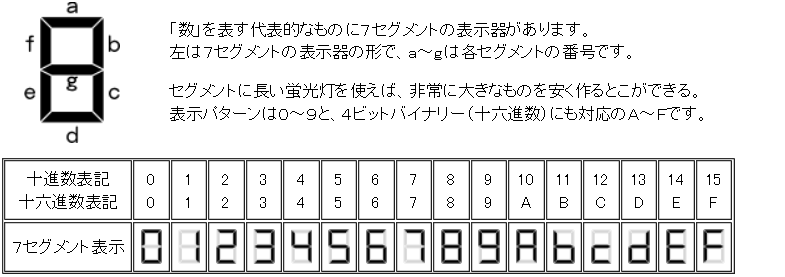
\includegraphics[width=15cm]{5-2.PNG}
\end{center}
そして、入力を表示する16進数、出力をそれぞれのセグメントa,b,c,d,e,f,gを表示させるならばTRUE、表示させないならばFALSEとするデコーダの入出力は以下の表のようになる。
\begin{center}
	デコーダの入出力
	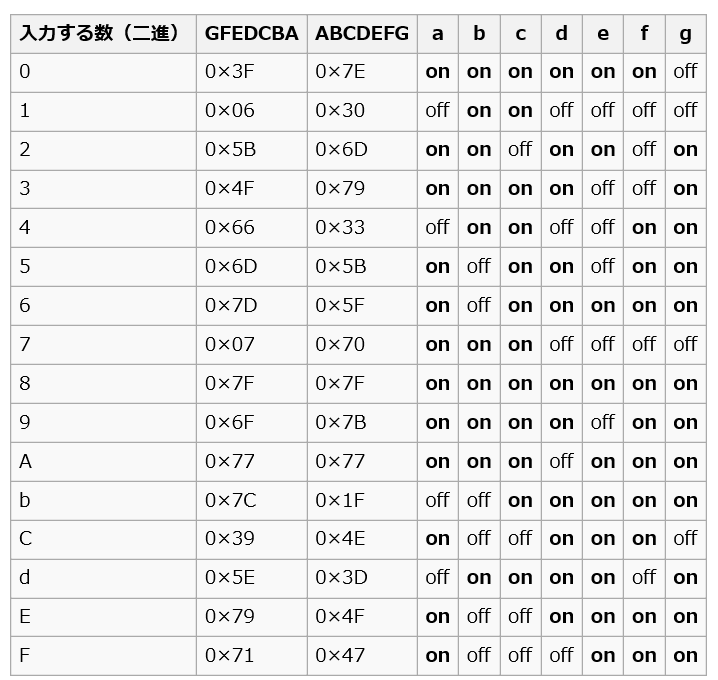
\includegraphics[width=15cm]{5-1.PNG}
\end{center}
これを元に、以下のようにモジュールを以下のソースコード\ref{work5sv}のように定義した。
\lstinputlisting[caption=$work5.sv$,label=work5sv]{5/work5.sv}
さらに、そのモジュールに対するテストベッドを以下のソースコード\ref{work5testbench}のように定義し、シミュレーションを実行した。
\lstinputlisting[caption=$testbench.sv$,label=work5testbench]{5/testbench.sv}
\subsubsection{結果}
シミュレーションを実行した結果、下の表のような波形が得られた。
\begin{center}
	課題5シミュレーション結果
	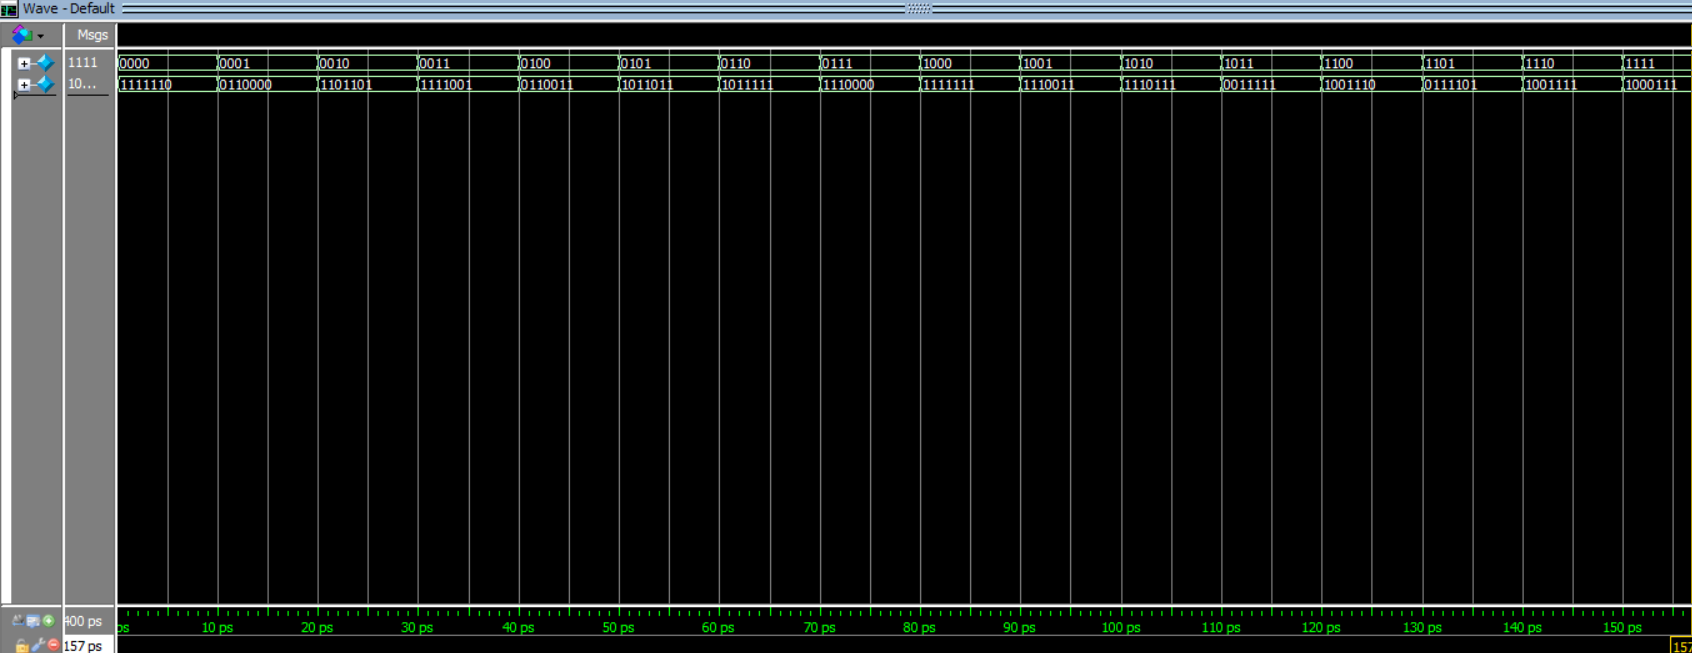
\includegraphics[width=15cm]{5-m.PNG}
\end{center}
\subsubsection{考察}
課題5では、SystemVerologを用いて16進7セグメントのデコーダを定義した。入力と出力に配列を用いて、配列のすべての要素に一気に値を入力する方法を知った。
\subsection{課題6}
\subsubsection{目的}
mux8という名の8:1マルチプレクサのモジュールを書き、これを使って論理関数$y = a \land \lnot b \lor \lnot \left( b \land c \right) \lor \lnot a \land b \land c$を計算する構造モジュールとそのテストヘッドを書き、シミュレーションで検証せよ。マルチプレクサの入力は$s\left[ 2:0 \right],d0,d1,d2,d3,d4,d5,d6,d7,$出力は$y$とする。
\subsubsection{道のり}
まず、8:1マルチプレクサの真理値表は以下の表\ref{Work6Mux8TruthTable}のようになる。
\begin{table}[ht]
	\begin{center}
		\caption{8:1マルチプレクサの真理値表}
		\label{Work6Mux8TruthTable}
		\begin{tabular}{|c|c|c|c|c|c|c|c|c|c|c||c|}
			\hline
			\multicolumn{11}{|c|}{入力} & \multicolumn{1}{|c|}{出力}\\	\hline\hline
			s[2]	&s[1]	&s[0]	&d0	&d1	&d2	&d3	&d4	&d5	&d6	&d7	&y\\	\hline\hline
			0	&0	&0	&0	&x	&x	&x	&x	&x	&x	&x	&0\\	\hline
			0	&0	&0	&1	&x	&x	&x	&x	&x	&x	&x	&1\\	\hline
			0	&0	&1	&x	&0	&x	&x	&x	&x	&x	&x	&0\\	\hline
			0	&0	&1	&x	&1	&x	&x	&x	&x	&x	&x	&1\\	\hline
			0	&1	&0	&x	&x	&0	&x	&x	&x	&x	&x	&0\\	\hline
			0	&1	&0	&x	&x	&1	&x	&x	&x	&x	&x	&1\\	\hline
			0	&1	&1	&x	&x	&x	&0	&x	&x	&x	&x	&0\\	\hline
			0	&1	&1	&x	&x	&x	&1	&x	&x	&x	&x	&1\\	\hline
			1	&0	&0	&x	&x	&x	&x	&0	&x	&x	&x	&0\\	\hline
			1	&0	&0	&x	&x	&x	&x	&1	&x	&x	&x	&1\\	\hline
			1	&0	&1	&x	&x	&x	&x	&x	&0	&x	&x	&0\\	\hline
			1	&0	&1	&x	&x	&x	&x	&x	&1	&x	&x	&1\\	\hline
			1	&1	&0	&x	&x	&x	&x	&x	&x	&0	&x	&0\\	\hline
			1	&1	&0	&x	&x	&x	&x	&x	&x	&1	&x	&1\\	\hline
			1	&1	&1	&x	&x	&x	&x	&x	&x	&x	&0	&0\\	\hline
			1	&1	&1	&x	&x	&x	&x	&x	&x	&x	&1	&1\\	\hline
		\end{tabular}
	\end{center}
\end{table}
これをもとに、8:1マルチプレクサを以下のソースコード\ref{Work6Mux8}のように定義した。
\lstinputlisting[caption=$mux8.sv$,label=Work6Mux8]{6/mux8.sv}
次に、このマルチプレクサを使って$y = a \land \lnot b \lor \lnot \left( b \land c \right) \lor \lnot a \land b \land c$を計算する構造モジュールを定義する。
この関数の真理値表は以下の表\ref{Work6TruthTable}のようになる。
\begin{table}[ht]
	\begin{center}
		\caption{課題6論理関数の真理値表}
		\label{Work6TruthTable}
		\begin{tabular}{|c|c|c||c|}
			\hline
			\multicolumn{3}{|c|}{入力} & \multicolumn{1}{|c|}{出力}\\	\hline\hline
			a	&b	&c	&y\\	\hline\hline
			0	&0	&0	&1\\	\hline
			0	&0	&1	&1\\	\hline
			0	&1	&0	&1\\	\hline
			0	&1	&1	&1\\	\hline
			1	&0	&0	&1\\	\hline
			1	&0	&1	&1\\	\hline
			1	&1	&0	&1\\	\hline
			1	&1	&1	&0\\	\hline
		\end{tabular}
	\end{center}
\end{table}
これをもとにして、モジュールwork6を以下のソースコード\ref{Work6SV}のように定義した。
\lstinputlisting[caption=$work6.sv$,label=Work6SV]{6/work6.sv}
さらに、このモジュールの動作を検証するテストベッドを以下のソースコード\ref{Work6TestBench}のように定義し、シミュレーションを実行した。
\lstinputlisting[caption=$testbench.sv$,label=Work6TestBench]{6/testbench6.sv}
\subsubsection{結果}
シミュレーションを実行した結果、以下のように真理値表通りの波形が得られた。
\begin{center}
	課題6シミュレーション結果
	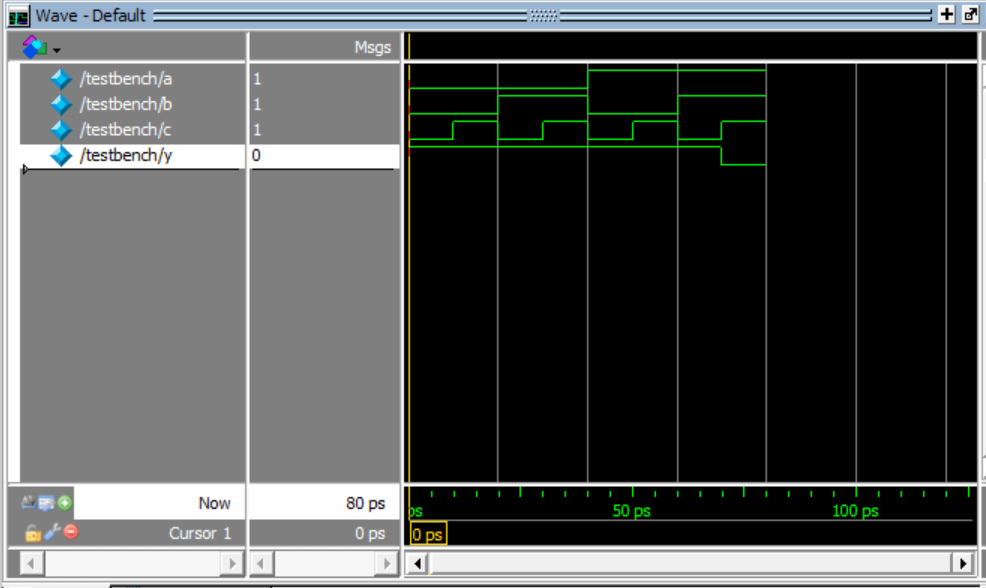
\includegraphics[width=15cm]{6-m.PNG}
\end{center}
\subsubsection{考察}
課題6では、8:1マルチプレクサのモジュールを定義して、そのモジュールを使用して簡単な回路を設計した。これにより、あるモジュールの回路の中に、別のモジュールの回路を埋め込む方法を知った。
\subsection{課題7}
\subsubsection{目的}
2:4デコーダのSystemVerilogモジュールとそのテストベッドを書き、シミュレーションで検証せよ。
\subsubsection{道のり}
まず、2:4デコーダの真理値表は以下の表\ref{Work7TruthTable}のようになる。
\begin{table}[ht]
	\begin{center}
		\caption{2:4デコーダの真理値表}
		\label{Work7TruthTable}
		\begin{tabular}{|c|c||c|c|c|c|}
			\hline
			\multicolumn{2}{|c|}{入力} & \multicolumn{4}{|c|}{出力}\\	\hline\hline
			x[0]	&x[1]	&y[0]	&y[1]	&y[2]	&y[3]\\	\hline\hline
			0	&0	&1	&0	&0	&0\\	\hline
			0	&1	&0	&1	&0	&0\\	\hline
			1	&0	&0	&0	&1	&0\\	\hline
			1	&1	&0	&0	&0	&1\\	\hline
		\end{tabular}
	\end{center}
\end{table}
これをもとにして、モジュールdecoderを以下のように定義した。
\lstinputlisting[caption=$work7.sv$,label=Work7SV]{7/work7.sv}
さらに、このモジュールの動作を検証するテストヘッドを以下のソースコード\ref{Work7TestBench}のように定義し、シミュレーションを実行した。
\lstinputlisting[caption=$testbench.sv$,label=Work7TestBench]{7/testbench.sv}
\subsubsection{結果}
シミュレーションを実行した結果、以下のように真理値表通りの波形が得られた。
\begin{center}
	課題6シミュレーション結果
	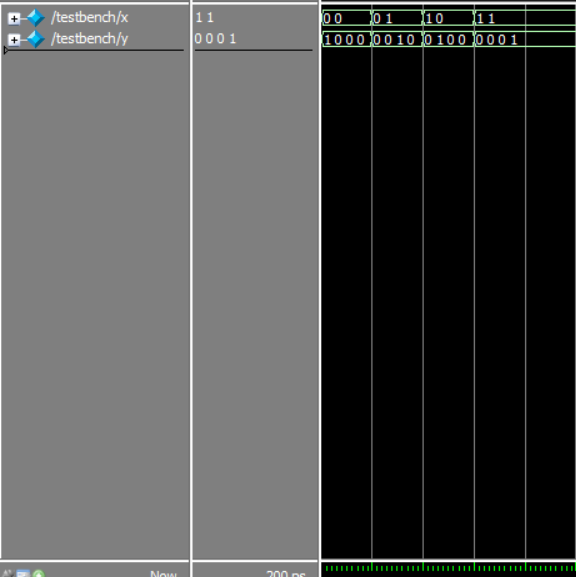
\includegraphics[width=15cm]{7-m.PNG}
\end{center}
\subsubsection{考察}
課題7では、2:4デコーダをSystemVerilogで設計し、その動作を検証するテストベッドを定義してシミュレーションを実行した。これにより、デコーダが複数の入力から特定の一つを選ぶ仕組みを理解することができた。
\subsection{課題9}
\subsubsection{目的}
ソースコード\ref{Work9FSM}のようなHDL記述で記述されるFSM(有限状態機械)の状態遷移図を描け。
\lstinputlisting[caption=$fsm1.sv$,label=Work9FSM]{9/fsm1.sv}
\subsubsection{道のり}
上のソースコード\ref{Work9FSM}を見て、まずこの機械が取りうる状態はS0,S1,S2,S3,S4の5種類である。初期状態はS2で、現在の状態と入力takenによって次の状態nextstateが決定していることがわかる。このようにソースコードを読んで、状態遷移図を書いた。
\subsubsection{結果}
以下の図のような状態遷移図を作ることができた。
\begin{center}
	課題9状態遷移図
	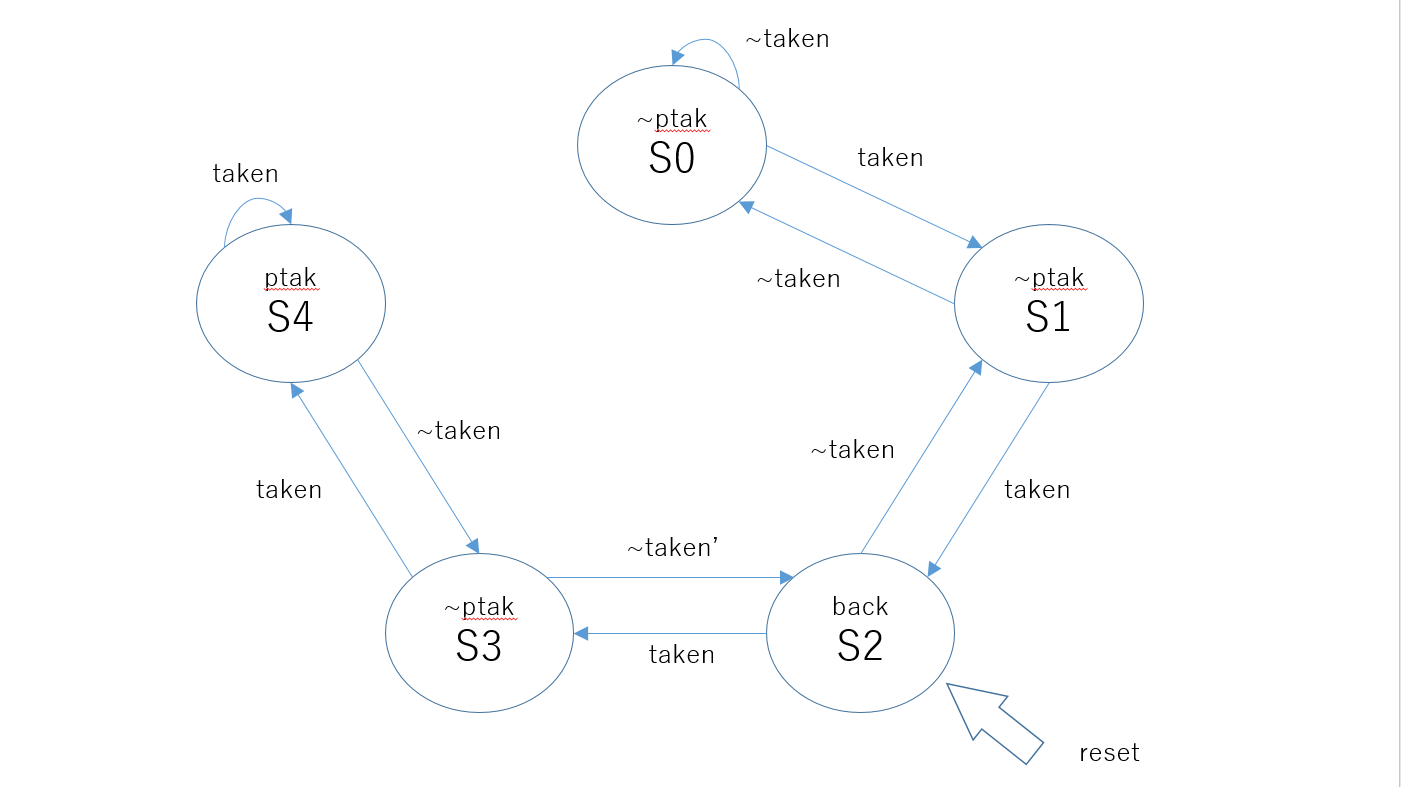
\includegraphics[width=15cm]{9.PNG}
\end{center}
\subsubsection{考察}
課題9では、SystemVerilogを読んで、それによって表現されている有限状態機械の状態遷移図を描いた。ソースコードを見てもそれがどんな機械なのかわかりにくかったが、状態遷移図にすることでわかりやすくなるように感じたが、複雑な回路になれば、状態遷移図にすると逆にわかりにくくなるのだろうと思う。
\subsection{課題11}
\subsubsection{目的}
JKフリップフロップのSystemVerilogモジュールとそのテストベッドを書き、シミュレーションで検証せよ。JKフリップフロップは入力として$clk,J,K$が、出力として$Q$がある。$J==K$なら、$clk$の立ち上がりエッジで$Q$は以前の状態を保持する。$clk$の立ち上がりエッジで、$J==1$ならば$Q$に$1$をセットし、$K==1$ならば$Q$に$0$をセットし、$J==K==1$ならば$Q$の値を反転させる。
\subsubsection{道のり}
まず、問題文に従って以下のソースコード\ref{Work11Jflipflop}でモジュールjflipflopを定義した。
\lstinputlisting[caption=$work11.sv$,label=Work11Jflipflop]{11/work11.sv}
次に、モジュールjflipflopの動作をテストするために以下のソースコード\ref{Work11TestBench}でテストベッドを定義し、シミュレーションを実行した。
\lstinputlisting[caption=$report11testbench.sv$,label=Work11TestBench]{11/report11testbench.sv}
\subsubsection{結果}
シミュレーションの結果、以下の図のような波形が得られた。
\begin{center}
	課題11シミュレーションの実行結果
	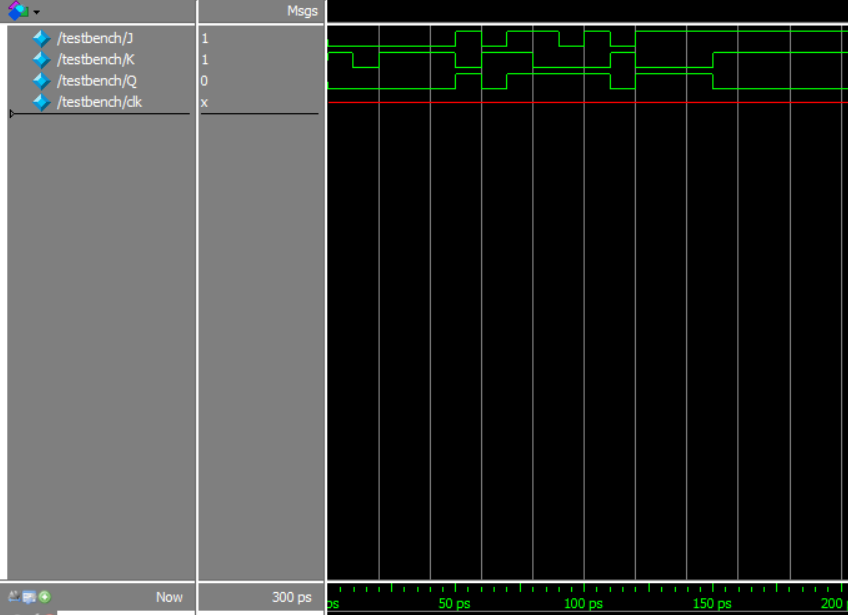
\includegraphics[width=15cm]{11-m.PNG}
\end{center}
\subsubsection{考察}
作成したモジュールjflipflopは入力$J$と$K$に応じて出力$Q$の値を出すが、$clk$の立ち上がりエッジを考慮していなかったために正しく動作するjflipflopを作成することはできなかった。
\subsection{課題12}
\subsubsection{目的}
入力はクロックの$clk$のみで、3ビットの出力のある3ビット8剰余Grayコードカウンタの有限状態マシンを設計せよ。
\subsubsection{道のり}
まず、Grayコードカウンタの定義に従って、以下のソースコード\ref{Work12GrayCodeCounter}でGrayコードカウンタを定義した。
\lstinputlisting[caption=$work12.sv$,label=Work12GrayCodeCounter]{12/work12.sv}
次に、その動作を検証するために以下のソースコード\ref{Work12TestBench}でテストベッドを定義し、シミュレーションを実行した。
\lstinputlisting[caption=$testbench.sv$,label=Work12TestBench]{12/testbench.sv}
\subsubsection{結果}
シミュレーションを実行した結果、以下の図のような波形を得ることができた。
\begin{center}
	課題12シミュレーションの実行結果
	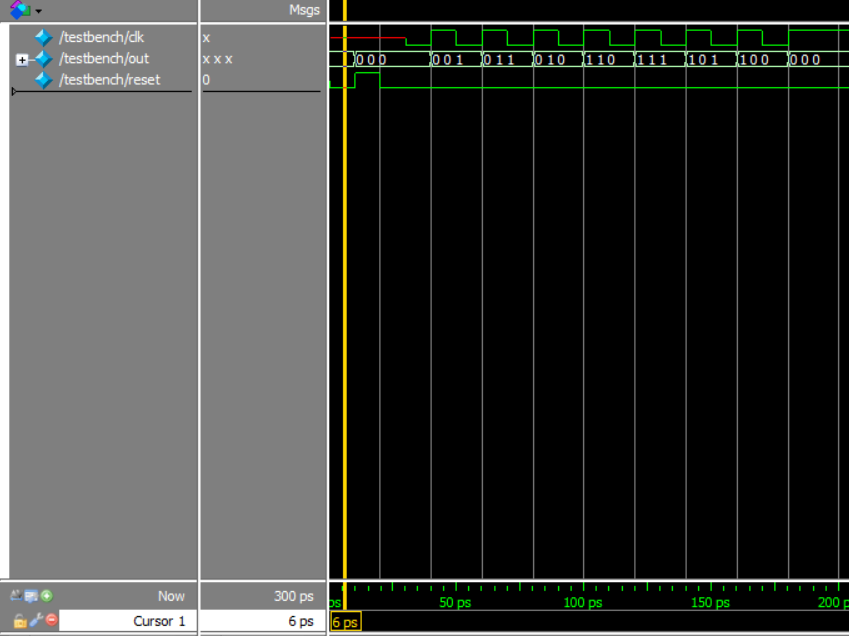
\includegraphics[width=15cm]{12-m-1.PNG}
\end{center}
\subsubsection{考察}
課題12では、Grayコードカウンタを設計し、SystemVerilogでの順序回路の設計のしかたを知った。
\section{実験の総括的なまとめ、感想}
今回の実験ではSystem Verilogの文法やModelSimの使い方をあまり理解できないまま進めていったのでとても苦戦し、時間がかかった。他のグループの人の助けも借りながらなんとか課題を完了させた。
\end{comment}
\end{document}

